
\subsection{Model 1: Beneficial and Harmful Content}

Users of a platform submit some large number of items of content. Each of these items generates some value for the speaker who posted it, for the platform, and for its listeners. It also potentially generates some harms for third parties: copyright infringement harms copyright owners, defamation harms the defamed, and so on. We are interested in the platform's responses to content of varying harmfulness, so we treat the benefits as fixed parameters and the harms as variable. We can model how the platform's responses change for different categories of content by changing the parameters.

The users of the platform submit some large number $n$ of items of content. Let the variable $x \in [0,n]$ range over the content. For each $x$, the platform has the option either to leave it up or to take it down. If the platform leaves it up, there are four effects:
\begin{itemize}
\item It generates fixed value $S \ge 0$ for the speaker who posted it.
\item It generates fixed value $P \ge 0$ for the platform.
\item It generates fixed value $L \ge 0$ for the listeners who read it, and for others in society.
\item It causes variable harm $h(x)$ for other members of society.
\end{itemize}
Although technically each item is discrete, for simplicity we treat the range $[0,n]$ as a continuum, so that $x$ and any functions of $x$ are continuous.\footnote{In the  case of a large platform, where the number of individual items is enormous, in the millions or even billions, a continuous approximation is quite reasonable.} We also assume that the items are ordered by increasing harmful harmfulness, so that $h(x)$ is a weakly increasing function of $x$. That is, if $x < y$, then $h(x) \le h(y)$. We also assume that the least harmful content is completely harmless, i.e. $h(0) = 0$. The following diagram illustrates for the case when the most harmful content is unambiguously harmful, i.e.  $h(n) > S + P + L$:

\begin{figure}[h]
	\centering
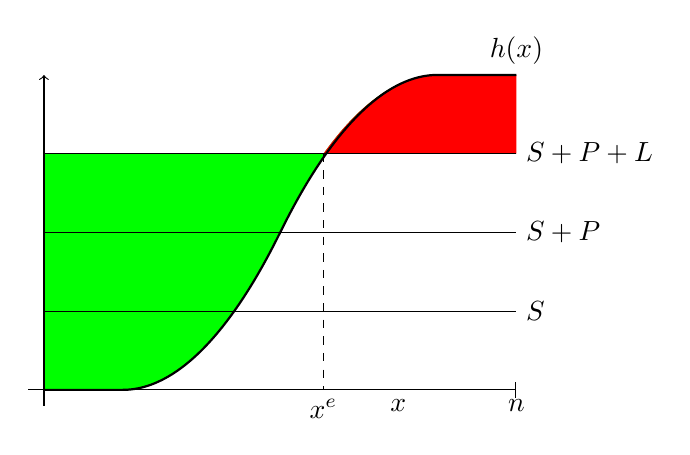
\begin{tikzpicture}[scale=1]
	\fill[green] (0,0) to (1,0) parabola (3,2) parabola bend +(2,2) (3.55,3) to (0,3) to (0,0);
	\fill[red] (3.55,3) parabola[bend at end] (5,4) to (6,4) to (6,3) to (3.55,3);
	\draw[-|] (-0.2,0) -- (3,0) -- node[below]{$x$} (6,0) node[below]{$n$}; 
	\draw[->] (0,-0.2) -- (0,4) node[above]{};
	\draw[thick] (0,0) to (1,0) parabola (3,2) parabola[bend at end] (5,4) to (6,4) node[above]{$h(x)$};

	\draw[thin] (0,1) to (6,1) node[right]{$S$};
%    \draw[dashed, thin] (1.75,1.5) -- (1.75,0) node[below]{$x^s$}; 

	\draw[thin] (0,2) to (6,2) node[right]{$S+P$};
%    \draw[dashed, thin] (1.75,1.5) -- (1.75,0) node[below]{$x^p$}; 
	
	\draw[thin] (0,3) to (6,3) node[right]{$S+P+L$};
	\draw[dashed, thin] (3.55,3) -- (3.55,0) node[below]{$x^e$}; 
	
\end{tikzpicture}
	\caption{Social benefits and harms of content}
	\label{fig:removal}
\end{figure}


The net benefit or harm to society of the content on the platform is given by the signed difference between $h(x)$ and $S+P+L$. The green region represents the content that is net beneficial, i.e. $S+P+L > h(x)$. The red region represents the content that is net harmful, i.e. $h(x) > S+P+L$. The diagram shows that there is a unique efficient outcome defined by setting a threshold $x^e$ defined by $h(x^e) = S + P + L$, in which all of the net beneficial content (with $x < x^e$) stays up and all of the net harmful content (with $x > x^e$) is removed.

In a standard tort-liability model, an actor chooses a level of activity that causes both private benefits and harms to identifiable victims. A regime of strict liability, in which the actor must compensate the victims for the harms they suffer, leads to an efficient outcome. And if there were a single actor that realized the full social value $S + P +L$ from the content $x$ that it leaves up, a strict liability regime requiring it to pay compensation $h(x)$ for the harms caused by that content would be efficient. 

In our model, this is the case when the platform captures all of 





% Figure here with constant P

The shaded area is the total value to users of posting their content to the platform. It has height $P$ and width $N$, for total value $PN$. This the value to users of having the platform, if it were free to them.

Now, consider the platform's incentives. For now, we assume that the platform can capture all of the value to users of posting their content. We also assume that the platform has infinite capacity, but incurs fixed costs $F$, which it must pay to operate all. Then the platform's profit if it operates is $PN - F$. The following diagram shows the platform's profits if it operates as a function of $N$.

% Diagram

It starts at $-F$ and crosses the $x$ axis at $N = F/P$. Beneath that level, the platform is unprofitable and will not operate at all, so that the value to society is $0$. Above that level, the platform recovers its costs and hosts all the content, so that the value to society is $PN - F $.(We must of course include the costs of operating the platform in the 

Because the platform captures all of the users' value, it fully internalizes all of the costs and benefits to society of operating. Thus, society's overall welfare function is the same as the platform's profits. If $PN < F$, the platform is a net negative because it costs more to operate than the value it delivers, and a regulator should prefer that it not operate. If $PN > F$, the platform is a net positive and a regulator should prefer it to operate. No regulation is required; the platform's incentives match the regulator's goals.

\subsection{Model 2: Harmful Content}
 
Now we consider the fact that some content is harmful. Suppose that \emph{some} of the items of content cause constant harm $H$ if the platform hosts them. In this model, we assume that everyone (including the regulator and the platform) knows which items these are. Thus, without loss of generality, \emph{we order the items of content by how harmful they are, from least harmful to most harmful}. Since the harm cause by harmful content is constant, this means we can define a step function $h(x)$:

\begin{equation}
h(x)=
\lt\{\begin{array}{ll}
	0 & \mbox{if $x>\hat{x}$}, \\
	H & \mbox{otherwise}.
\end{array}\rt.
\end{equation}

In the case where $H>P$, each item of harmful content is a net negative for society. This results in the following diagram:

% Step function h

The shaded area on the left, with area $\hat{x}P$, consists of the beneficial content. The shaded area on the right, with area $(N - \hat{x})(H-P)$, consists of the harmful content. The socially efficient outcome is achieved when the platform hosts only the beneficial content.

We introduce new notation for the idea that the platform can set a threshold: for $x$ beneath the threshold, the platform leaves the content up, for $x$ greater than the threshold, the platform takes the content down. We define $x^e$ (the $e$ is for ``efficient'') to be the cutoff point at which the threshold is efficient. It is obvious by inspection that in this model $x^e = \hat{x}$ -- subject to the same condition as above, that it is efficient for the platform to operate at all. If $\hat{x}P < F$, the game is not worth the candle, and society prefers that the platform not operate at all. Otherwise, social welfare is $\hat{x}P - F$.

Now consider the platform's incentives, which can diverge from the regulator's goals because the platform internalizes $P$ (the value of content to users) but not $H$ (the harm caused by the content).  In the absence of liability, the platform will host \emph{all} the content, beneficial and harmful, for net profits of $NP - F$, as above. But now social welfare equals $\hat{x}P - F - (N - \hat{x})(H - P)$, which is smaller than the social welfare at $x^e$ because of the extra term.

What should the regulator do? One option is to prohibit all platforms. This is an improvement on the no-regulation baseline in the case where $\hat{x}P - (N - \hat{x})(H - P) - F < 0$. But it is not efficient in the case where $\hat{x}P > F$, and it would be profitable to have  platform operate.

Instead -- and this is the classic starting point of law-and-economics analysis of tort liability -- the regulator should impose liability on the platform for the harmful content it carries. This fixes the platform's incentives by making it internalize both the costs and the benefits of its conduct. One rule, of strict liability, holds the platform liable for all the harm it causes. Under this rule, for $x <\hat{x}$, the platform has marginal profit of $P$, which is positive, so it will add more content until it reaches $\hat{x}$. But for $x > \hat{x}$, the platform's marginal profit is $P - H$, which is negative, so it will remove content until it reaches $\hat{x}$.  Introducing the notation $x^*$ for the platform's optimum, we say that $x^* = x^e = \hat{x}$.

Another classic rule, of negligence, sets a level of care $x^n$ and imposes liability $L$ for each item of content if the platform operates above that level. But here, the efficient level of care is just $x^n = \hat{x}$ again, so as long as $L>P$, the platform will again set its threshold at the efficient point of $\hat{x}$ and the two rules are effectively identical.

Before moving on, consider another variation in the parameters. We have been discussing the case where $H > P$. But there is also the case where $H < P$ -- i.e., the content is beneficial on net, but causes harms the platform does not internalize.

% diagram

Here, the efficient level of operation is $x^e = N$, i.e. society prefers that all of the content remain available. Under the no-liability baseline, the platform will do just that. But if the regulator imposes liability, matters are more complicated. If the platform must pay compensation $H$ for each item of harmful content, its profits are $NP - (N - \hat{x})(P - H) - F $. This can cause the platform to shut down if the need to pay compensation makes it unviable, i.e., when 

\begin{equation}
NP - (N - \hat{x})(P - H) < F <  NP
\end{equation}

% Diagram platform's profits as a function of $x^c$.

This concern puts regulators to a choice: in some cases, \emph{without the profits attributable to harmful content, a platform cannot operate to serve beneficial content}. In this model with $H < P$, the problem is avoidable, because even the content that causes harms is still beneficial on net. But we will soon see models in which the tradeoff is sharper.


\subsection{Model 3: Variably Harmful Content}

In the previous model, $h(x)$ was a step function: some content is harmless with $h(x) = 0$ and some content is harmful with $h(x) = H$. Now we extend this model by making $h(x)$ a more general function. Once again, we order the content by increasing harmfulness, so that $h(x) \le h(y)$ for $x < y$. We also assume that $h(0) =0$ (i.e., there is some content that is unambiguously good). To simplify the case analysis, we also require that $h(N) => P$, i.e. there is some content that is unambiguously harmful. Now the diagram of the benefits and harms from content looks like the following:

% diagram

The regulator would prefer the content to carry all content $x$ for which $h(x) <P$ and to remove all content for which $h(x) > P$. By the intermediate value theorem, there is some point $x^e$ for which $h(x^e) = P$. Because $h(x)$ is weakly increasing, it follows that $h(x) \le P$ for all $x< x^e$ and $h(x) \ge P$ for all $x > x^e$. Thus, the same result as in the previous model follows: the regulator wants the platform to allow content exactly up to $x = x^e$. The actual expression for social welfare is more complicated because $h(x)$ is no longer constant. If the platform leaves up all content through $\hat{x}$, then the social welfare function is

\begin{equation}
\int_{0}^{\hat{x}} P - h(x) dx - F
\end{equation}

In the absence of liability, however, the platform fails to internalize the harms. Its profit function is 

\begin{equation}
\int_{0}^{\hat{x}} P dx - F
\end{equation}

which it maximizes by setting $\hat{x} = N$, i.e. leaving up all content. Once again, the regulator can impose strict liability. If it does so, then the platform's profit function equals the social welfare function, and the platform will set the efficient threshold $\hat{x} = x^e$. Similarly, the regulator could impose a threshold-based liability $h(x)$ starting at at threshold $x^n$. In this case, the platform's marginal profit will be $P$ for $x < x^n$ and $P - h(x)$ for $x > x^n$, and the platform has efficient incentives for $x^n = x^e$. 

The difference between the two regimes is that in the former, the platform compensates those who are harmed for $x < x^e$; in the latter it does not. In diagram XXX, this compensation is the difference between the two shaded regions 1 and 2, and just the upper one. In the case where

XXX equation

the choice can affect the viability of the platform, just as in the previous model.

\subsection{Model 4: Positive Externalities}

Next, we add in another important fact about content: it creates positive externalities that are not fully captured by the platform. There are several overlapping reasons why this is so:

\begin{itemize}
\item The platform may not be able to price access in ways that captures all of the surplus it creates for its users.
\item Information is a public good. Once it has been shared on the platform, it can be shared further in ways the platform cannot perfectly track or monetize.
\item A typical platform has at least some competition, so it will price beneath the level it would as a monopolist.
\end{itemize}

We model these externalities by adding an additional term $\delta$ to the value created by carrying a given piece of content. Like $P$, we assume that $\delta$ is constant across all content. Thus, each piece of content carried generates $P$ in value for the platform and $\delta$ in value for society at large, for a total of $P + \delta$. Again for simplicity, assume that $h(N) > P + \delta$. Now the diagram looks like:

% diagram with P, P + \delta, and h(x)

Assuming the platform operates, the efficient level of moderation is at $x^e$ where $h(x^e) = P + \delta$. With immunity, the platform undermoderates, just as before, and hosts all content. Under strict liability, the platform moderates at $x^*$ such that $h(x^*) = P$, which is to the left of $x^e$, i.e., the platform undermoderates. The shaded triangle in diagram XXX illustrates the lost social value: this is content that is positive-value for society (because $h(x) < P + \delta$ but which is unprofitable for the platform to host (because $h(x) > P$). Compare the result under a threshold liability rule: the regulator will set the threshold at $x^e$ rather than at $x^e$, leading the platform to set its cutoff at $x^e$.




\subsection{Model 5: Unknown Content}

All of the previous models assumed perfect information about the harms caused by content. It is time to relax this assumption, because several of the most interesting and important consequences for content moderation depend on the difficulty of distinguishing between beneficial and harmful content.

We return to a fixed harm: each item of harmful content causes harm $H$. But now we make the \emph{probability} of harm variable. The function $\lambda(x)$ represents the probability that the item of content $x$ is harmful. That is, with probability $\lambda(x)$, item $x$ causes harm $H$, and with probability $1 - \lambda(x)$, it causes harm $0$. We assume that the platform and regulator have perfect information about $H$ and $\lambda()$, that $\lambda(x)$ is weakly increasing in $x$, and that there is some content known to be harmless and some known to be harmful, i.e. $\lambda(0) = 0$ and $\lambda(N) = 1$. The following diagram illustrates:

% diagram

This diagram should look familiar. It is the same as diagram XXX, except that the harm curve is now labeled $\lambda(x)H$ rather than $h(x)$. But the shape of the curves are the same. Each individual piece of content $x$ is either harmful or not with probability $\lambda(x)$, but in the continuous limit of an infinitely large $H$, this is the same as if the content in the neighborhood of $x$ is all equally harmful with harm $\lambda(x)$.

In particular, the regulator and platform have exactly the same welfare and utility functions as before.  If the platform leaves up all content through $\hat{x}$, then the social welfare function is

\begin{equation}
\int_{0}^{\hat{x}} P - \lambda(x)H dx - F
\end{equation}

so that social optimum where the marginal harm and marginal benefit from additional content exactly cancel is at $x^e$ such that $P = \lambda(x^e)H$. As before, however, the platform's profit function in the absence of liability is

\begin{equation}
\int_{0}^{\hat{x}} P dx - F
\end{equation} 

which is again maximized for $\hat{x} = N$. The same argument as above shows that either strict liability for all harms caused or liability for all harmful content above the threshold $x^e$ is efficient -- subject to the constraint that in the former case the platform must be profitable, i.e. $\int_0^{x^e} P dx = x^eP \ge F$.


\subsection{Model 6: Platform Investigation}

The next model is the same as the previous one -- content causes harm $H$  with weakly increasing probability $\lambda(x)$ -- except that the platform now has a new option. It can incur a cost of $c > 0$ to investigate an item of content and determine with certainty whether it is harmful. Note that it only makes sense for the platform to investigate if the results will affect the platform's decision. Otherwise, the platform could save $c$ by skipping the investigation and doing what it would have done anway.


% diagram



\begin{figure}[ht]
	\centering
\begin{tikzpicture}[scale=1]
%    \fill[green] (0,0) to (.5,0) parabola (2.15,1) to (0,1) to (0,0);
%    \fill[red] (2.15,1) parabola[bend at end] (4.5,3) to (5,3) to (5,1) to (2,1);
	\drawaxes{factory production}
	\harmfunction{harm to society}
	\revenuefunction{factory revenue}
	\drawarrows[.25]{revenue}{harm}[green,-{Triangle}]{0}{2}
	\drawarrows[.25]{revenue}{harm}[red, -{Triangle}]{2}{5} 
	\xelevel
%    \draw[dashed, thin] (1.75,1.5) -- (1.75,0) node[below]{$x^p$}; 
	
%    \draw[thin] (0,3) to (5,3) node[right]{$S+P+L$};
%    \draw[dashed, thin] (3.55,3) -- (3.55,0) node[below]{$x^e$}; 
	
\end{tikzpicture}
	\caption{Non-Speech Torts}
	\label{fig:factory}
\end{figure}









\begin{econ}{Widget production}{fig:factory1}
  \drawaxes{production}{\$}
  \revenueline{revenue}
  \dropline{6}{1.5}{$\hat{x}$}
  \fill[pattern=vertical lines, pattern color=green] (0,0) to (6,0) to (6,1.5) to (0,1.5) to (0,0);
\end{econ}

\begin{econ}{Social welfare for widgets}{fig:factory2}
  \drawaxes{production}{\$}
  \fill[pattern=vertical lines, pattern color=green] (0,0) to (1,0) parabola (4.1,1.5) to (0,1.5) to (0,0);
  \fill[pattern=vertical lines, pattern color=red] (4.1,1.5) parabola bend +(-3,-1.5) (5,2.5) parabola[bend at end] (9,5) to (10,5) to (10,1.5) to (4.1,1.5);
  \revenueline{revenue}
  \harmfunction{harm}
  \xe
\end{econ}

\begin{econ}{Strict liability is efficient for widgets}{fig:factory3}
  \drawaxes{production}{\$}
  \fill[pattern=vertical lines, pattern color=green] (0,0) to (1,0) parabola (4.1,1.5) to (0,1.5) to (0,0);
  \fill[pattern=vertical lines, pattern color=green] (0,0) to (1,0) parabola (4.1,1.5) to (0,1.5) to (0,0);
  \revenueline{revenue}
  \harmfunction{harm}
  \xexhat
\end{econ}


\begin{econ}{Speech production}{fig:speech1}
  \drawaxes{production}{\$}
  \dropline{6}{2.5}{$\hat{x}$}
  \fill[pattern=vertical lines, pattern color=green] (0,0) to (6,0) to (6,1.5) to (0,1.5) to (0,0);
  \fill[pattern=dots, pattern color=blue] (0,1.5) to (6,1.5) to (6,2.5) to (0,2.5) to (0,1.5);
  \revenueline{revenue}
  \spilloverline{social value}
\end{econ}

\begin{econ}{Social welfare for speech}{fig:speech2}
  \drawaxes{production}{\$}
  \fill[pattern=vertical lines, pattern color=green] (0,0) to (1,0) parabola (5,2.5) to (0,2.5) to (0,0);
  \fill[pattern=vertical lines, pattern color=red] (5,2.5) parabola [bend at end] (9,5) to (10,5) to (10,2.5) to (5,2.5);
  \revenueline{revenue}
  \spilloverline{social value}
  \harmfunction{harm}
  \dropline{5}{2.5}{$x^e$}
\end{econ}



\begin{econ}{Strict liability chills valuable speech}{fig:speech3}
  \drawaxes{production}{\$}
  \fill[pattern=vertical lines, pattern color=green] (0,0) to (1,0) parabola (4.1,1.5) to (0,1.5) to (0,0);
  \fill[pattern=dots, pattern color=blue] (0,1.5) to (4.1,1.5) to (4.1,2.5) to (0,2.5) to (0,1.5);
  \fill[pattern=north west lines, pattern color=red] (4.1,1.5) parabola bend +(-3,-1.5) (5,2.5) to (4.1,2.5) to (4.1,1.5);
  \revenueline{revenue}
  \spilloverline{social value}
  \harmfunction{harm}
  \dropline{4.1}{1.5}{$\hat{x}$}
  \dropline{5}{2.5}{$x^e$}
\end{econ}



\begin{econ}{Imperfect information about harm}{fig:imperfect1}
  \drawaxes{}{}
  \fill[pattern=fivepointed stars, pattern color=red] (0,0) to (1,0) parabola (5,2.5) parabola[bend at end] (9,5) to (10,5) to (10,0) to (0,0);
  \fill[pattern=sixpointed stars, pattern color=green] (0,0) to (1,0) parabola (5,2.5) parabola[bend at end] (9,5) to (10,5) to (0,5) to (0,0);
  \draw[thick] (.425,0) to (.425,5) to (.625,5) to (.625,0) to (.425,0) node[below]{$\lambda = 0$};
  \draw[thick] (4.025,0) to (4.025,5) to (4.225,5) to (4.225,0) to (4.025,0) node[below]{$\lambda = .3$};
  \draw[thick] (9.15,0) to (9.15,5) to (9.35,5) to (9.35,0) to (9.15,0) node[below]{$\lambda = 1$};
\end{econ}



\begin{econ}{Strict liability chills valuable speech}{fig:imperfect2}
  \drawaxes{production}{\$}
  \fill[pattern=vertical lines, pattern color=green] (0,0) to (1,0) parabola (4.1,1.5) to (0,1.5) to (0,0);
  \fill[pattern=dots, pattern color=blue] (0,1.5) to (4.1,1.5) to (4.1,2.5) to (0,2.5) to (0,1.5);
  \fill[pattern=north west lines, pattern color=red] (4.1,1.5) parabola bend +(-3,-1.5) (5,2.5) to (4.1,2.5) to (4.1,1.5);
  \revenueline{revenue}
  \spilloverline{social value}
  \harmline{$H$}
  \draw[name path=harm, thick] (0,0) to (1,0) parabola (5,2.5) parabola[bend at end]   (9,5) to (10,5);
  \node at (7.5,4) {$\lambda(x)H$};
  \dropline{4.1}{1.5}{$\hat{x}$}
  \dropline{5}{2.5}{$x^e$}
\end{econ}


\begin{pgfecon}{Decreasing platform revenue}{fig:test1}
  \lambdaplot
  \plotvalue{welfare}{4}{15}{$s(x)$}
  \plotvalue{profit}{2}{20}{$p(x)$}
  \dropline{4.28}{1.65}{$x^*$};
  \dropline{5.4}{3}{$x^e$};
  \addplot [pattern= dots, pattern color = blue] fill between [of = profit and welfare, soft clip={domain=0:4.28}];
  \addplot [pattern= north east lines, pattern color = red] fill between [of = welfare and lambda, soft clip={domain=4.28:5.4}];
  \addplot [pattern= grid, pattern color = green] fill between [of = profit and lambda, soft clip={domain=0:4.28}];
\end{pgfecon}



% \begin{econ}{Non-Speech Torts}{fig:factory2}
%   \drawaxes{widget production}{\$}
%   \harmfunction{harm to society}
%   \revenueline{factory revenue}
%   \drawarrows[.25]{revenue}{harm}[green,-{Triangle}]{0}{4}
%   \drawarrows[.25]{revenue}{harm}[red, -{Triangle}]{4}{10} 
%   \xe
% \end{econ}




\subsection{Traditional Liability}

A widget factory must decide how many widgets to make. As it increases production, it must use increasingly hazardous manufacturing techniques, with two effects.  On the one hand, this increased production is less and less profitable: the cost to make each widget rises. On the other hand, the increased production has worse and worse environmental effects: the amount of pollution the factory emits increases.

Mathematically, we say that the factory chooses a level of production $\hat{x} \in [0,n]$. The factory's marginal revenue per unit of widgets sold is a weakly nonincreasing function $p(x)$ (i.e. $x < y$ implies $p(x) \ge p(y)$), and the the marginal environmental harm caused per unit of widgets sold is a weakly nondecreasing function $h(x)$ (i.e. $x < y$ implies $h(x) \le h(y)$). For simplicity of exposition, we assume that the first widgets are profitable and harmless (i.e. $p(0) > 0$ and $h(0) = 0$ and that the last possible widgets cause more harm than good (i.e. $h(n) > p(n)$).  The factory has fixed costs $F$, so the factory's profits are given by 
\begin{equation}
\int_{0}^{\hat{x}} p(x) dx - F
\end{equation}
if it operates and total social welfare is given by:
\begin{equation}
\int_{0}^{\hat{x}} p(x) - h(x) dx - F
\end{equation}
If the factory cannot operate profitably, it shuts down, and both its profit and social welfare are $0$.






\begin{pgfecon}{A platform chooses its moderation level in the presence of harm}{fig:harm1}
  \lambdaplot
  \plotvalue{profit}{2}{20}{$p(x)$}
  \plotvalue{welfare}{3.5}{15}{$s(x)$}
  \dropline{3.5}{3.25}{$\hat{x}$};
  \dropline{5.1}{2.6}{$x^e$};
  %\draw[dashed, thin] (8, 0) node[below left]{$x^*=x^e$};
  % \addplot [pattern= dots, pattern color = blue] fill between [of = profit and welfare, soft clip={domain=0:4.28}];
  % \addplot [pattern= north east lines, pattern color = red] fill between [of = welfare and lambda, soft clip={domain=4.28:5.4}];
  \addplot [pattern= grid, pattern color = green] fill between [of = profit and lambda, soft clip={domain=0:3.5}];
  \addplot [pattern= dots, pattern color = blue] fill between [of = welfare and profit, soft clip={domain=0:3.5}];
  \addplot [pattern= north east lines, pattern color = red] fill between [of = lambda and axis, soft clip={domain=0:3.5}];
\end{pgfecon}




As Figure \ref{fig:host3} illustrates, the positive spillover means that the platform will systematically overmoderate compared to the social optimum. As before, the green gridded region is the platform' profits. The blue dotted region above it is the positive spillovers for society created by the content the platform hosts. But the red striped region represents content that would have been socially beneficial, but which was not privately profitable for the platform to host.



We refer to this legal regime as \emph{blanket immunity}. 
